\section{Uzyskane wyniki}\label{rozdzial_wyniki}
\newcommand{\imageSize}{1.15}
\subsection{Parametry zadowolenia oraz pobudzenia}
Zależność pomiędzy odpowiedziami oczekiwanymi przez sieć, a~jej rzeczywistymi odpowiedziami, w~przypadku dobrze nauczonej i~działającej sieci powinna być zbliżona do liniowej. Biorąc to pod uwagę, przedstawiono wykresy, których jedna oś wskazuje oczekiwaną wartość parametru, a~druga rzeczywistą wartość parametru w celu zaobserwowania czy występuję liniowość, co też uczyniono, a efekty można zaobserwować na rysunkach \ref{arousal} oraz \ref{valence}. Jak można zauważyć, istnieje pewna korelacja dla obu parametrów. W~celu określenia konkretnych wartości liczbowych wskazujących na korelację możemy posłużyć się współczynnikiem korelacji liniowej zmiennych $x$ oraz $y$, który wyraża się wzorem:
\begin{equation}
\rho_{xy} = \frac{cov(x,y)}{\sigma_x \sigma_y},
\end{equation}
gdzie $\sigma_x$, $\sigma_y$ są odchyleniami standardowymi odpowiednio $x$ oraz $y$, natomiast $cov(x,y)$ jest kowariancją i określamy ją wzorem:
\begin{equation}
cov(x,y) = \overline{xy} - \overline{x}*\overline{y},
\end{equation}
gdzie $\overline{xy}$, $\overline{x}$, $\overline{y}$ są kolejno wartościami średnimi $xy$, $x$ oraz $y$.
Obliczone współczynniki korelacji przedstawiono w~tabeli \ref{table:coeff}.
Zaobserwowana korelacja nie jest zbyt duża, niemniej jednak widzimy wyraźny związek pomiędzy odpowiedzią sieci neuronów, a~wartościami pobudzenia oraz zadowolenia wyznaczonymi przez badane osoby. Biorąc pod uwagę subiektywny
charakter oceny nastroju przez człowieka, jak również fakt, że sieć neuronowa używała tylko 11 cech uzyskanych z danego utworu muzyki, jest to wynik świadczący tym, że przedstawiony system do pewnego stopnia reprodukuje subiektywne oceny ludzi.
\begin{table}
\centering
\begin{tabular}{|c|c|c|}
\hline
 parametr & zadowolenie & pobudzenie \\ 
\hline
 współczynnik korelacji & $0.66$ & $0.55$ \\  
\hline 
\end{tabular}
\caption{Współczynniki korelacji liniowych parametrów zadowolenia oraz pobudzenia} \label{table:coeff}
\end{table}


\begin{figure}[ht!]
\centering
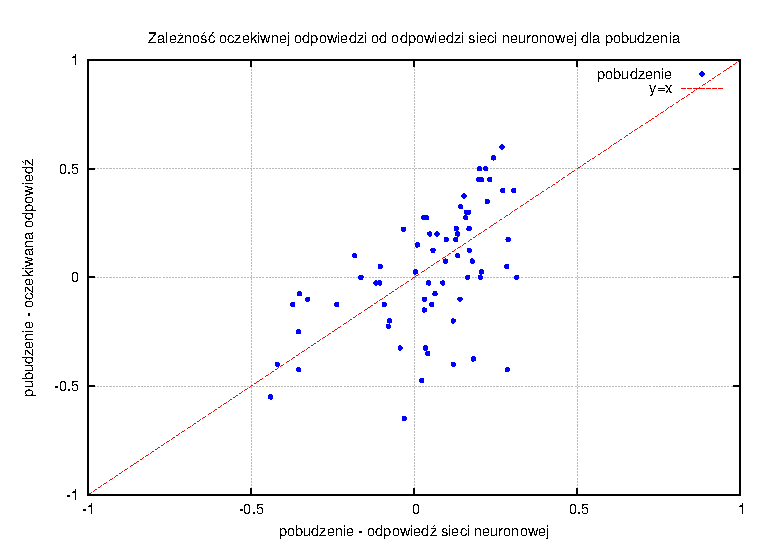
\includegraphics[scale=\imageSize]{res/arousal.eps}
\caption{Zależność oczekiwanej odpowiedzi od odpowiedzi sieci neuronowej dla parametru pobudzenia\label{arousal}}
\end{figure}

\begin{figure}[ht!]
\centering
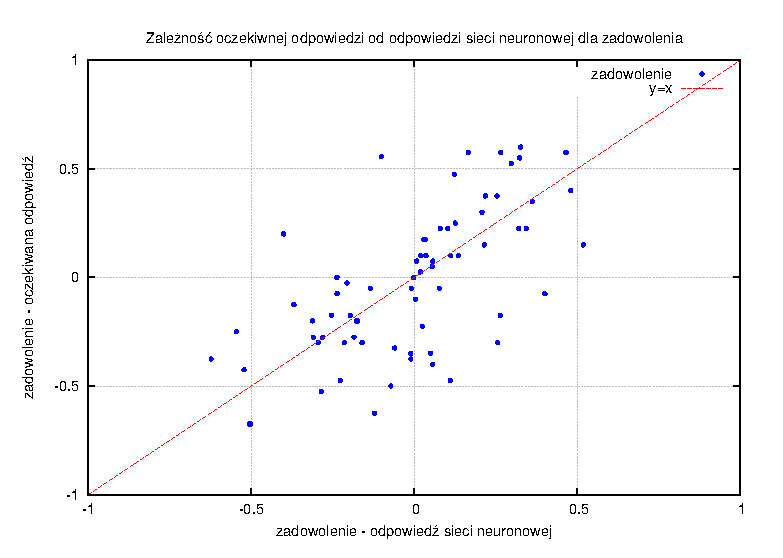
\includegraphics[scale=\imageSize]{res/valence.eps}
\caption{Zależność oczekiwanej odpowiedzi od odpowiedzi sieci neuronowej dla parametru zadowolenia\label{valence}}
\end{figure}


\subsection{Zależność nastroju od cech dźwiękowych}\label{rozdzial_zaleznosc}
Pod uwagę zostało wziętych 11 cech dźwiękowych, które mają różny wpływ na subiektywny nastrój reprezentowany przez utwór muzyczny. W~tym rozdziale przeanalizowana jest zależność wartości parametrów zadowolenia oraz pobudzenia od wartości cech dźwiękowych. 


%%%%%%%%%%%%%%%%%%%%%%%%%%%%%%%%%%%%%%%%%%%%%%%%%%%%%%%%
\paragraph{Wskaźnik zmiany znaku}\mbox{}\\
\begin{minipage}{\textwidth}
Rysunek \ref{wykresCrossRate} przedstawia zależność wskaźnika zmiany znaku od subiektywnej oceny zadowolenia oraz pobudzenia. Możemy zaobserwować tendencję, że wraz ze wzrostem wartości tego wskaźnika wzrasta również wartość obu parametrów - zadowolenia jak i~pobudzenia. Nie jest to jednak znaczący wzrost.
\end{minipage}
\begin{figure}[ht!]
\centering
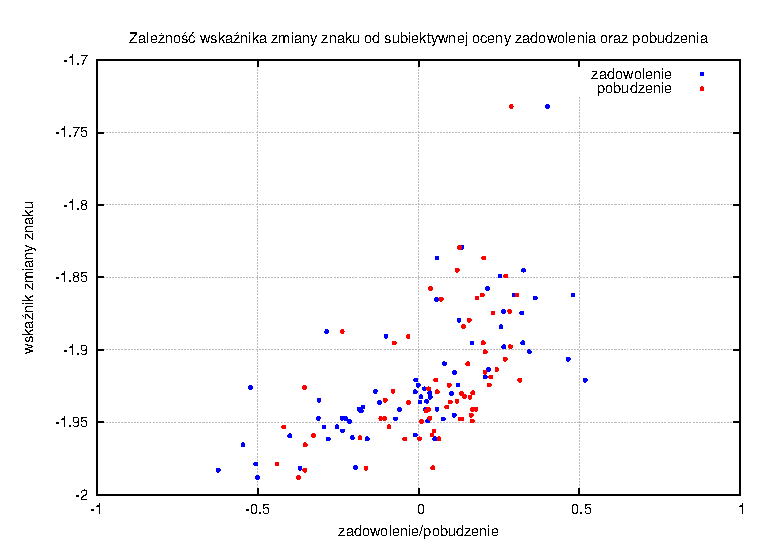
\includegraphics[scale=\imageSize]{res/crossRate.eps}
\caption{Zależność wskaźnika zmiany znaku od subiektywnej oceny zadowolenia (punkty niebieskie) oraz pobudzenia (punkty czerwone)\label{wykresCrossRate}}
\end{figure}
%%%%%%%%%%%%%%%%%%%%%%%%%%%%%%%%%%%%%%%%%%%%%%%%%%%%%%%%
\paragraph{Wskaźnik zmian}\mbox{}\\
Podobnie jak w przypadku wskaźnika zmiany znaku, oba parametry - zadowolenie oraz pobudzenie wzrastają nieznacznie wraz ze wzrostem wskaźnika zmian, ale wzrost ten jest nieznaczny. Wykres przedstawiony jest na rysunku \ref{wykresOnset}.
\begin{figure}[ht!]
\centering
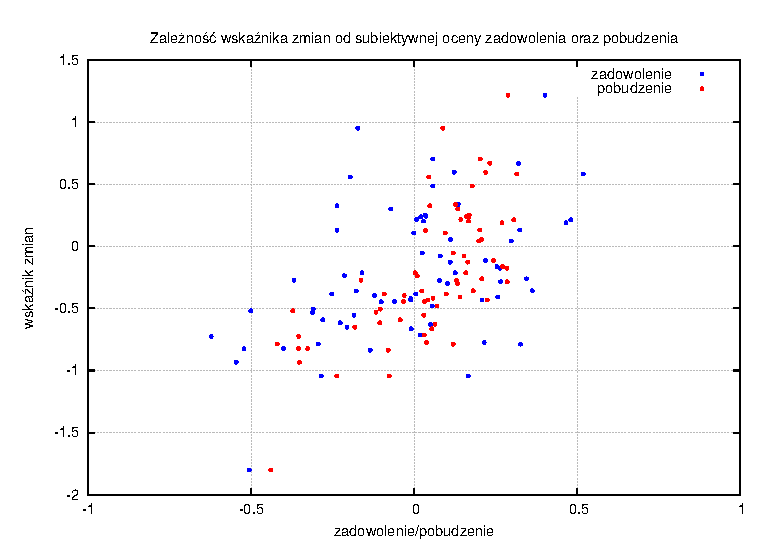
\includegraphics[scale=\imageSize]{res/onset.eps}
\caption{Zależność wskaźnika zmian od subiektywnej oceny zadowolenia (punkty niebieskie) oraz pobudzenia (punkty czerwone)\label{wykresOnset}}
\end{figure}
%%%%%%%%%%%%%%%%%%%%%%%%%%%%%%%%%%%%%%%%%%%%%%%%%%%%%%%%
\paragraph{Złożoność spektralna}\mbox{}\\
Zależność parametrów wskazujących na emocje od złożoności spektralnej została przedstawiona na rysunku \ref{wykresComplexity}. Obserwując wykres trudno mówić o~jakiejkolwiek korelacji. Zdecydowana większość wartości wydaje być się losowo rozrzucona.
\begin{figure}[ht!]
\centering
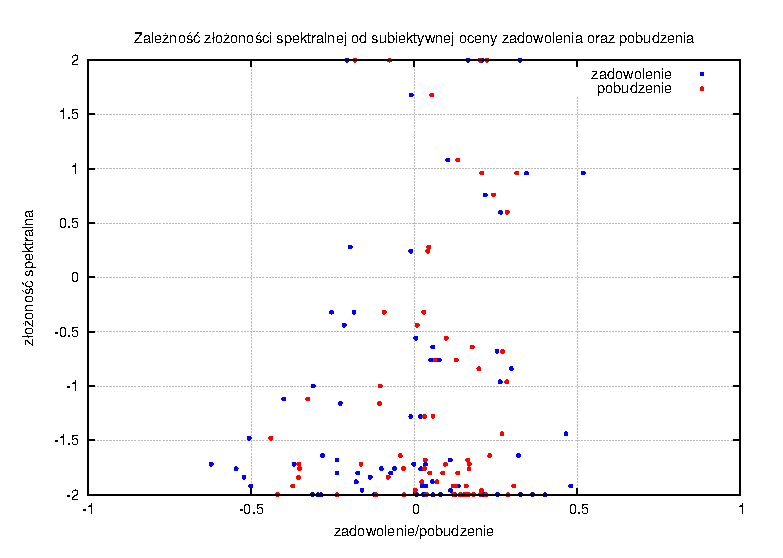
\includegraphics[scale=\imageSize]{res/complexity.eps}
\caption{Zależność złożoności spektralnej od subiektywnej oceny zadowolenia (punkty niebieskie) oraz pobudzenia (punkty czerwone)\label{wykresComplexity}}
\end{figure}


%%%%%%%%%%%%%%%%%%%%%%%%%%%%%%%%%%%%%%%%%%%%%%%%%%%%%%%%
\paragraph{Środek masy widma}\mbox{}\\
W~przypadku środka masy widma możemy zauważyć nieznaczny związek pomiędzy zmianą wartości środka widma, a~parametrami zadowolenia oraz pobudzenia. Zostało to przedstawione na rysunku \ref{wykresCentroid}.
\begin{figure}[ht!]
\centering
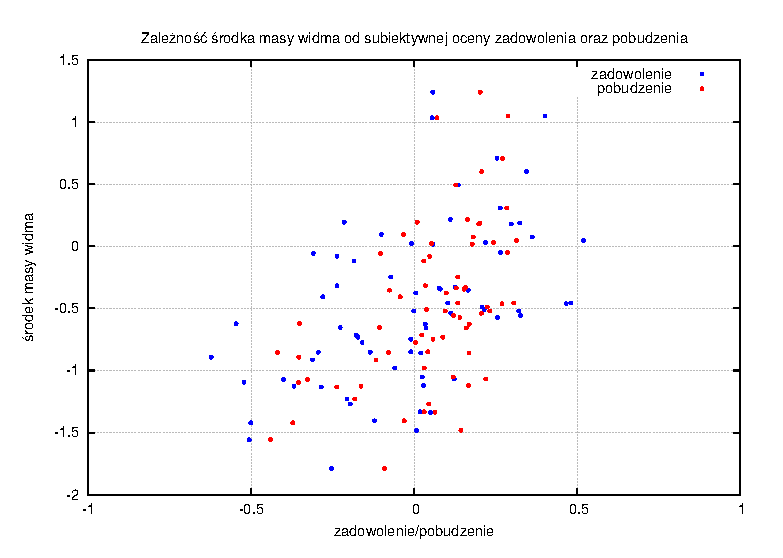
\includegraphics[scale=\imageSize]{res/centroid.eps}
\caption{Zależność środa masy widma od subiektywnej oceny zadowolenia (punkty niebieskie) oraz pobudzenia (punkty czerwone)\label{wykresCentroid}}
\end{figure}
%%%%%%%%%%%%%%%%%%%%%%%%%%%%%%%%%%%%%%%%%%%%%%%%%%%%%%%%
\paragraph{Współczynnik skośności widma}\mbox{}\\
Jeśli chodzi o~współczynnik skośności widma możemy zaobserwować, że przy wyższych jego wartościach parametry bardzo nieznacznie mogą być zwiększone, co jednak także nie jest wyraźne i~przedstawia się na wykresie \ref{wykresSkewness}.
\begin{figure}[ht!]
\centering
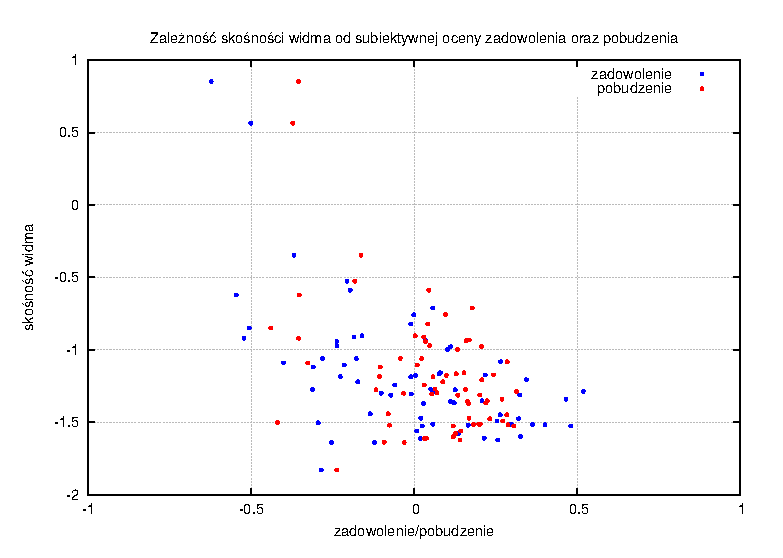
\includegraphics[scale=\imageSize]{res/skewness.eps}
\caption{Zależność skośności widma od subiektywnej oceny zadowolenia (punkty niebieskie) oraz pobudzenia (punkty czerwone)\label{wykresSkewness}}
\end{figure}
%%%%%%%%%%%%%%%%%%%%%%%%%%%%%%%%%%%%%%%%%%%%%%%%%%%%%%%%
\paragraph{Kurtoza widma}\mbox{}\\
Kurtoza widma według wykresu \ref{wykresKurtosis} nie wydaje się mieć większego wpływu na wartości parametrów zadowolenia oraz pobudzenia.
\begin{figure}[ht!]
\centering
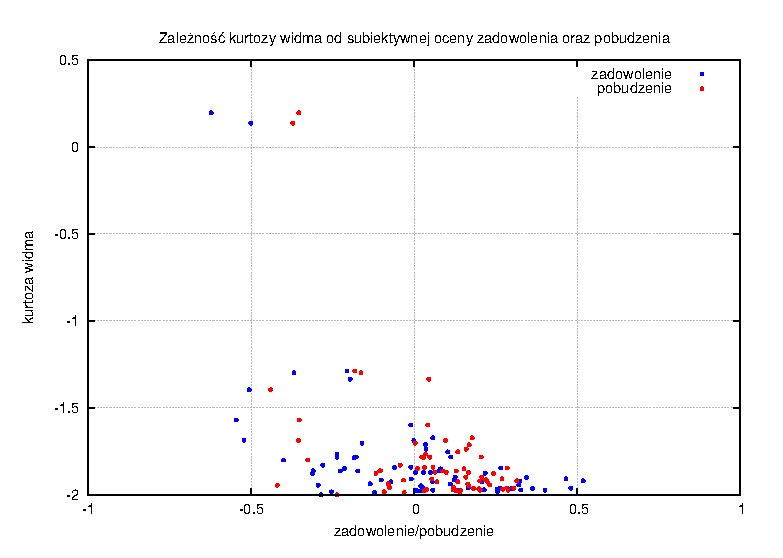
\includegraphics[scale=\imageSize]{res/kurtosis.eps}
\caption{Zależność kurtozy widma od subiektywnej oceny zadowolenia (punkty niebieskie) oraz pobudzenia (punkty czerwone)\label{wykresKurtosis}}
\end{figure}
%%%%%%%%%%%%%%%%%%%%%%%%%%%%%%%%%%%%%%%%%%%%%%%%%%%%%%%%
\paragraph{Rozrzut spektralny}\mbox{}\\
Rozrzut spektralny przedstawiony na wykresie \ref{wykresSpread} wydaje się być względnie znaczącym czynnikiem w~ocenie parametrów nastroju muzyki w~stworzonym systemie. Oba z~nich wzrastają w~przypadku wzrosty wartości tej cechy dźwięku.
\begin{figure}[ht!]
\centering
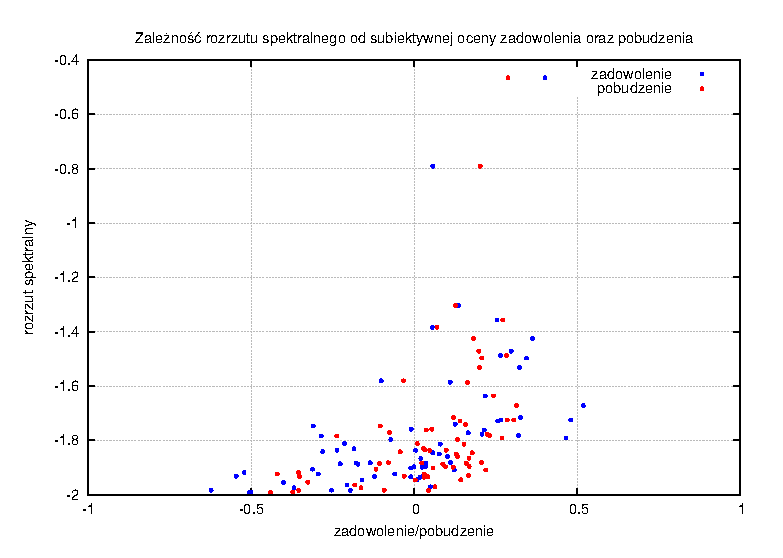
\includegraphics[scale=\imageSize]{res/spread.eps}
\caption{Zależność rozrzutu spektralnego od subiektywnej oceny zadowolenia (punkty niebieskie) oraz pobudzenia (punkty czerwone)\label{wykresSpread}}
\end{figure}
%%%%%%%%%%%%%%%%%%%%%%%%%%%%%%%%%%%%%%%%%%%%%%%%%%%%%%%%
\paragraph{\emph{Roll-off} widma}\mbox{}\\
Zależność \emph{Roll off}u widma od parametrów pobudzenia oraz zadowolenia nie wskazuje na większą korelację (patrz Rys.~\ref{wykresRollOff}).
\begin{figure}[ht!]
\centering
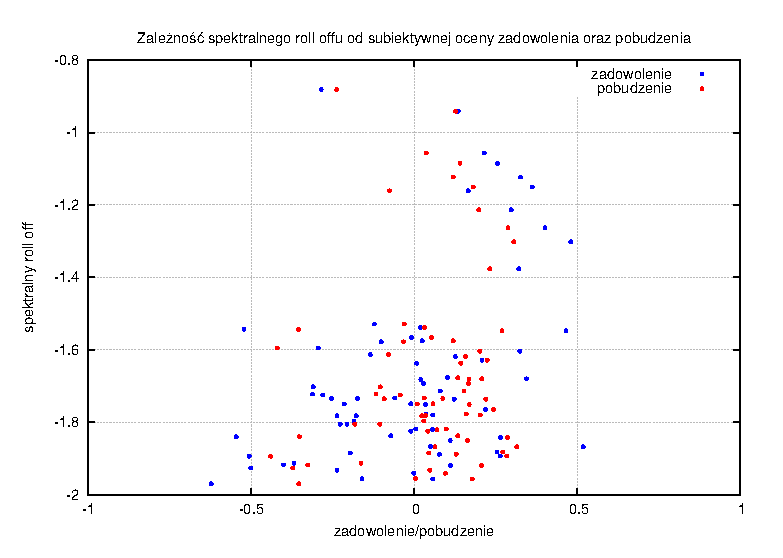
\includegraphics[scale=\imageSize]{res/rollOff.eps}
\caption{Zależność spektralnego \emph{roll off}'u od subiektywnej oceny zadowolenia (punkty niebieskie) oraz pobudzenia (punkty czerwone)\label{wykresRollOff}}
\end{figure}
%%%%%%%%%%%%%%%%%%%%%%%%%%%%%%%%%%%%%%%%%%%%%%%%%%%%%%%%
\paragraph{Płaskość spektralna}\mbox{}\\
Na wykresie \ref{wykresFlatness} przedstawiony został wpływ parametru płaskości spektralnej na parametry pobudzenia oraz zadowolenia. Również i~w~tym przypadku nie widać większych korelacji.
\begin{figure}[ht!]
\centering
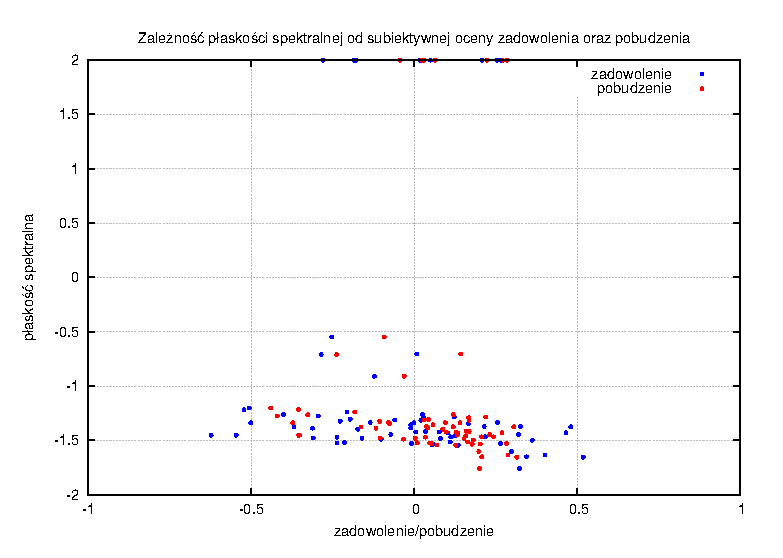
\includegraphics[scale=\imageSize]{res/flatness.eps}
\caption{Zależność płaskości spektralnej od subiektywnej oceny zadowolenia (punkty niebieskie) oraz pobudzenia (punkty czerwone)\label{wykresFlatness}}
\end{figure}

%%%%%%%%%%%%%%%%%%%%%%%%%%%%%%%%%%%%%%%%%%%%%%%%%%%%%%%%
\paragraph{Dysonans}\mbox{}\\
Podobnie jak w przypadku płaskości spektralnej nie istnieje większa korelacja pomiędzy parametrami nastroju muzyki, a~dysonansem, co wizualizuje wykres\ref{wykresDissonance}.
\begin{figure}[ht!]
\centering
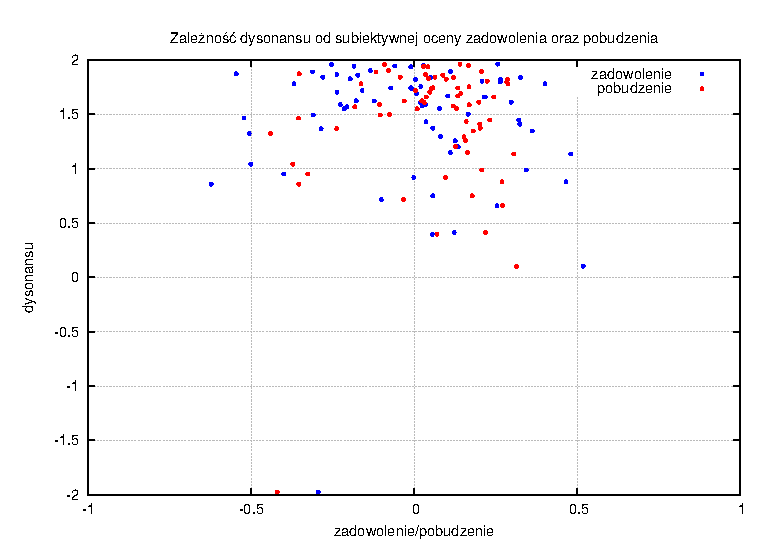
\includegraphics[scale=\imageSize]{res/dissonance.eps}
\caption{Zależność dysonansu od subiektywnej oceny zadowolenia (punkty niebieskie) oraz pobudzenia (punkty czerwone)\label{wykresDissonance}}
\end{figure}

%%%%%%%%%%%%%%%%%%%%%%%%%%%%%%%%%%%%%%%%%%%%%%%%%%%%%%%%
\paragraph{Skala}\mbox{}\\
W~tabeli \ref{table:scale} zostały przedstawione średnie wartości pobudzenia oraz zadowolenia dla skali muzycznych majorowej oraz minorowej, które jednak zbliżone są bardzo do siebie w przypadku obu skal. Sugeruje to, że ta cecha dźwiękowa nie była dobrym wskaźnikiem jeśli chodzi o~parametry pobudzenia oraz zadowolenia. 
\begin{table}
\centering
\begin{tabular}{|c|c|c|}
\hline
 skala & minorowa (molowa) & majorowa (durowa) \\ 
\hline
 wartość średnia dla zadowolenia & $0.02 \pm 0.25$ & $-0.08 \pm 0.30$ \\  
\hline 
 wartość średnia dla pobudzenia & $0.06 \pm 0.19$ & $0.03 \pm 0.19$ \\  
\hline 
\end{tabular}
\caption{Wartości średnie dla skali muzycznej wraz z odchyleniem standardowym} \label{table:scale}
\end{table}
\paragraph{Podsumowanie}\mbox{}\\
Obserwując wykresy dla poszczególnych cech dźwiękowych nie jest trudno dojść do wniosku, że nie wszystkie z~nich mają wpływ na parametry nastroju muzyki, a~te które mają, nie są silnymi zmiennymi. Tłumaczy to niezbyt wysoką korelację przedstawioną w~tabeli \ref{table:coeff}. Analiza utworów została przeprowadzona powtórnie, ale biorąc pod uwagę tylko te cechy, które korelowały z~wartościami pobudzenia oraz zadowolenia czyli: wskaźnik zmiany znaku, wskaźnik zmian, środek masy widma, skośność spektralną oraz rozrzut spektralny. Otrzymane rezultaty przedstawia tabela \ref{table:coeff2} oraz wykresy \ref{arousal2} i \ref{valence2}. Jak widać, usunięcie kilku zmiennych i pozostawienie tylko znaczących cech nie wpłynęło w~wyraźny sposób na wyniki reprezentowane przez współczynniki korelacji. Świadczy to o~tym, że na końcowy wynik efektywny wpływ ma tylko 5 pozostawionych cech.

\begin{table}
\centering
\begin{tabular}{|c|c|c|}
\hline
 parametr & zadowolenie & pobudzenie \\ 
\hline
 współczynnik korelacji & $0.54$ & $0.58$ \\  
\hline 
\end{tabular}
\caption{Współczynniki korelacji liniowych parametrów zadowolenia oraz pobudzenia} \label{table:coeff2}
\end{table}

\begin{figure}[ht!]
\centering
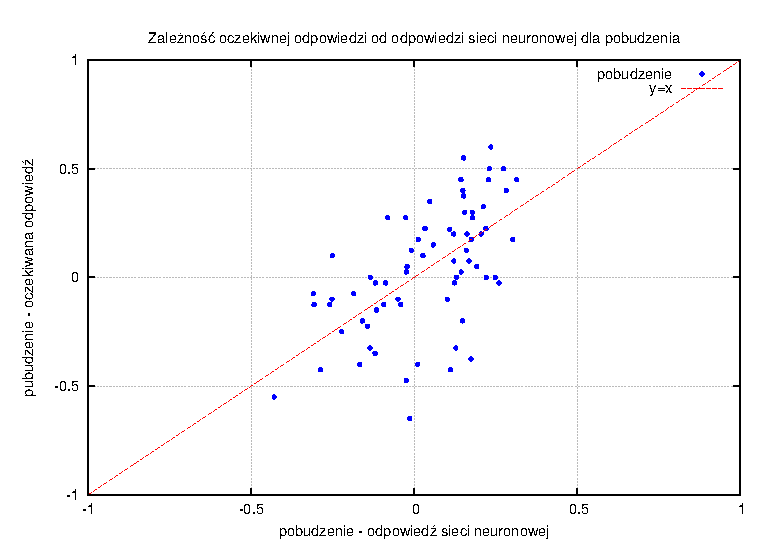
\includegraphics[scale=\imageSize]{res/arousal2.eps}
\caption{Zależność oczekiwanej odpowiedzi od odpowiedzi sieci neuronowej dla parametru pobudzenia\label{arousal2}}
\end{figure}

\begin{figure}[ht!]
\centering
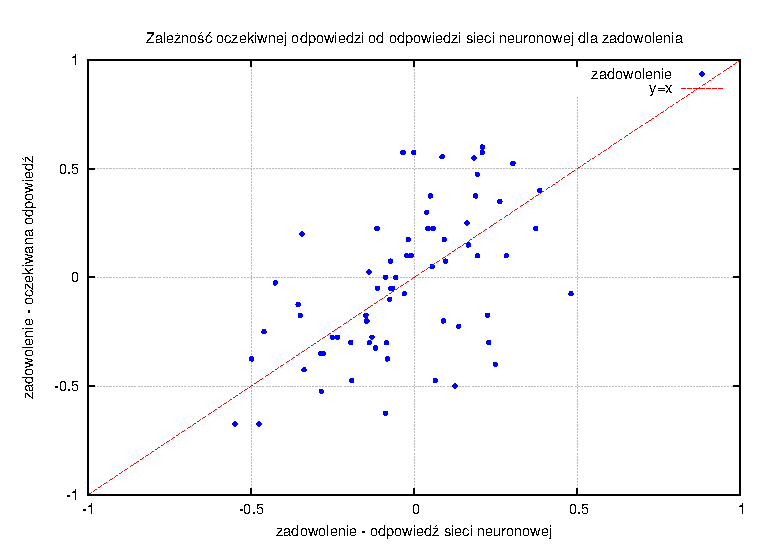
\includegraphics[scale=\imageSize]{res/valence2.eps}
\caption{Zależność oczekiwanej odpowiedzi od odpowiedzi sieci neuronowej dla parametru zadowolenia\label{valence2}}
\end{figure}





